\documentclass[journal]{IEEEtran}

\usepackage[spanish]{babel}
\usepackage[utf8]{inputenc}
\usepackage[T1]{fontenc}
\usepackage{graphicx}
\usepackage{amssymb}
\usepackage{amsmath}
\usepackage{amsthm}
\usepackage{booktabs}
\usepackage{gensymb}
\usepackage{stfloats}
\usepackage{float}
\usepackage{nccmath}
\usepackage{caption}
\usepackage{url}
\usepackage{listings}

\title{\textbf{SWITCHES y VLANs}}

\author{Redes LAN \\
	\textit{Profesor:} Luis Fernando Díaz Cadavid\\ 
	\textit{Monitores:} Juan José Jaramillo Granada - 814034 \\
	Kevin Leonardo Cerpa Campanella - 814017 \\
	Universidad Nacional de Colombia - Sede Manizales}

\date{}

\begin{document}
\maketitle

\section{\textbf{Descripción}}
En esta práctica se introducirán los conocimientos necesarios para configurar un Switch correctamente en packet tracer, e introducir el concepto de VLAN y aplicarlo a la configuración del Switch

%\section{Hablando de Protocolos}
%Un protocolo es
%	\subsection{TELNET}
%	El protocolo \textit{TELNET} es un protocolo que perimite simular el receptor como una máquina conectada a la misma red para acceder a ella y manejarla remotamente a través de una IP.
%	\subsection{SSH}
%	El protocolo \textit{SSH (Secure SHel)} proporciona	un inicio de sesión remoto similar al Telnet, excepto que utiliza servicios de red más seguros. El SSH proporcionaautenticación de contraseña más potente que Telnet y usa encriptación cuando transporta datos de una sesión. 	De esta manera se mantienen en privado la ID del usuario, la contraseña y los detalles de la sesión de administración. Se recomienda utilizar el protocolo SSH en lugar del Telnet, siempre que sea posible.
%	\subsection{TCP/IP}
%	El protocolo \textit{TCP/IP} consiste en

\section{\textbf{¿Por qué se debe configurar un dispositivo?}}
En escencia es por seguridad, ya que equipos como Routers, Switches, al ser dispositivos tan importantes para la comunicación en una red no cualquier persona debe acceder a ellos, ya que puede hacer un cambio, puede adquirir datos de la red de la compañía, puede restringir el acceso y un ejemplo muy claro de esto es un banco o un agente de control del estado. \\
Fuera de esto también se pueden realizar cambios para mejorar la red, a través de sus puertos, de las ventajas que nos brindan, y para esto debemos conocer como funciona y cuales son su utilidad

\section{\textbf{SWITCH}}
Un Switch que traducido al español para el área de red es un \textit{Conmutador} lo cual es un dispositivo cuya función es añadir funcionalidades, mejoras, control a una red LAN, además de interconectar los dispositivos que hagan parte de esta red.
Fotoooooooooooooooo

\section{\textbf{¿Qué es una VLAN?}}
Una VLAN (Virtual Local Area Network) es una red de área local virtual que se pueden crear en dispositivos de red. \\
Algunas ventajas que obtenemos al crear VLANs son:
\begin{enumerate}
	\item Seguridad
	\item Reducción de costos
	\item Superior rendimiento (broadcast domain)
\end{enumerate}

Los tipos de VLANs más comunes que se pueden encontrar en el diseño y administración de redes son:
\begin{itemize}
	\item VLAN de Datos
	\item VLAN Predeterminada
	\item VLAN de Admnistración
	\item VLAN Nativa
	\item VLAN de Voz
\end{itemize}

\section{\textbf{Manejo de Switches en Packet Tracer}}

\subsection{\textbf{Comandos Básicos}}
Entramos a Packet Tracer y agregamos al área de trabajo en Switch Cisco 2960, luego vamos a la pestaña CLI y observaremos algo semejante a:

\begin{figure}[ht]
	\centering
	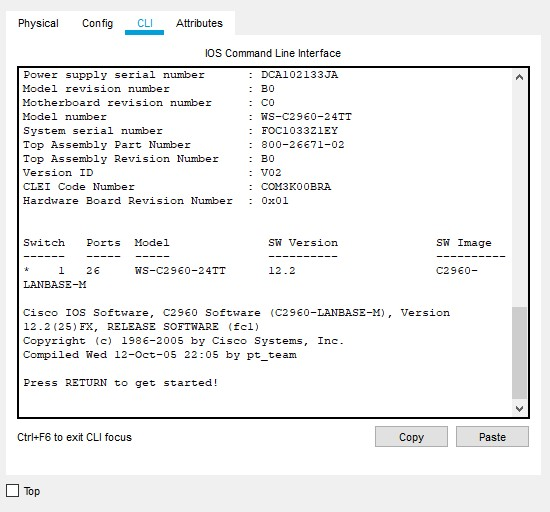
\includegraphics[scale=0.5]{cli.jpg}
	\caption{CLI en Packet Tracer}
\end{figure}

¿Qué es el CLI?, CLI (Command Line Interface) es una interfaz de linea de comandos que permite configurar un dispostivo de red. Allí podremos cambiar las configuraciones y poder tener control del dispositivo.

Para habilitar la entrada de comandos ingresamos la siguiente instrucción:
\begin{lstlisting}[frame=single]
enable
\end{lstlisting}

Existe tres tipos de usuarios dentro del CLI, los cuales son:
\begin{enumerate}
	\item Usuario Normal ( $>$ )
	\item Usuario Privilegiado ($\#$), es un modo de solo lectura. \\
	Para saber los comandos que se pueden usar en modo privilegiado ingresamos el siguiente comando "\textit{?}"
	\item Modo de configuración global ("nombre\_del\_dispositivo"(config)$\#$)
\end{enumerate}

Para ver todas las configuraciones actuales de Switch ingresamos el comando:
\begin{lstlisting}[frame=single]
show running-config
\end{lstlisting}

Para entrar al usuario de modo de configuración global ingresamos:
\begin{lstlisting}[frame=single]
configure terminal
\end{lstlisting}

\subsection{\textbf{Configuraciones Básicas}}
Cuando se administan redes se requiere de poder realizar una configuración remota al Switch, siempre por el protocolo SSH, por lo tanto en estas configuraciones básicas mostradas a continuación se incluyen también las configuraciones básicas que se requieren tanto para el Switch como para la conexión SSH
Para configurar un Switch debemos ingresar al usuario de configuración global.
\begin{enumerate}
	
	\item Asignar un nombre al Switch
	\begin{lstlisting}[frame=single]
hostname "nombre"
	\end{lstlisting}
	
	\item Asignar una contraseña
	\begin{lstlisting}[frame=single]
enable secret "password"
	\end{lstlisting}
	
	\item Encriptar la contraseña
	
	\begin{lstlisting}[frame=single]
service password-encryption
	\end{lstlisting}
	
	\item Agergar un mensaje de inicio, suele ser un mensaje de acceso restringido, ya que no todas las personas deben de tener acceso al switch
	\begin{lstlisting}[frame=single]
banner motd #"mensaje"#
	\end{lstlisting}
	
	\item Crear VLAN
	\begin{lstlisting}[frame=single]
vlan "#VLAN"
	\end{lstlisting}
	
	\item Luego se nos abre el entorno de configuración de VLAN (config-vlan) y le agregamos un nombre
	\begin{lstlisting}[frame=single]
name "nombre_VLAN"
	\end{lstlisting}
	
	\item Salimos del entorno de configuración de VLAN, esto con el comando \textit{exit} y debemos de activar la VLAN creada, esto con el comando:
	\begin{lstlisting}[frame=single]
interface vlan "#vlan"
	\end{lstlisting} 
	
	\item Creamos el número de VLANs requeridas para la red
	
	\item Luego de creadas las VLANs debemos asignar los puertos físicos que van a estar asociados a cada VLAN, debemos acceder al puerto o rango de puertos que vamos a configurar en la interfaz, para esto ingresamos el siguiente comando:
	\begin{lstlisting}[frame=single]
interface fa0/"#p_inicio-#p_fin"
	\end{lstlisting}
	"\textit{fa}" es la abreviatura que IOS asocia al puerto FastEthernet y de igual manera "\textit{gi}" es la abreviatura para el puerto GigaEthernet
	
	\item Luego habilitamos los puertos en modo de acceso:
	\begin{lstlisting}[frame=single]
switchport mode access
	\end{lstlisting} 
	
	\item Y asignamos este puerto o rango de puertos a una VLAN previamente creada:
	\begin{lstlisting}[frame=single]
switchport access "#vlan"
	\end{lstlisting}
	
	\item Y especificamos que los puertos estén encendidos:
	\begin{lstlisting}[frame=single]
no shutdown
	\end{lstlisting}
	Se recomienda que todo puerto o interfaz que no va a ser utilizado esté apagado según la distribución de la red y la ubicación de sus respectivos dispositivos de red.
	Para entrar a la interfaz de un solo puerto solo quitamos la palabra \textit{range} e introducimos el puerto a deshabilitar, y dentro del rango o puerto introducimos el comando \textit{shutdown}
	
	\item Luego nos regresamos al modo de configuración global y guardamos los cambios hechos con el comando:
	\begin{lstlisting}[frame=single]
do write
	\end{lstlisting}
	
	 \item Por último revisamos que las configuraciones estén guardadas correctamente con el comando \textit{show running-config} en modo privilegiado 
	 
\end{enumerate}

\subsection{\textbf{Confirmar Configuración}}
Luego de realizada una configuración básica debemos de revisar que la configuración está correcta, para esto agregamos dispositivos a la red y los conectamos a diferentes puertos asociados a diferentes VLANs y no debe haber comunicación entre dispositivos de diferentes VLANs. \\ \\

En la siguiente imágen se propone una red de prueba con tres VLANs diferentes:

\begin{figure}[ht]
	\centering
	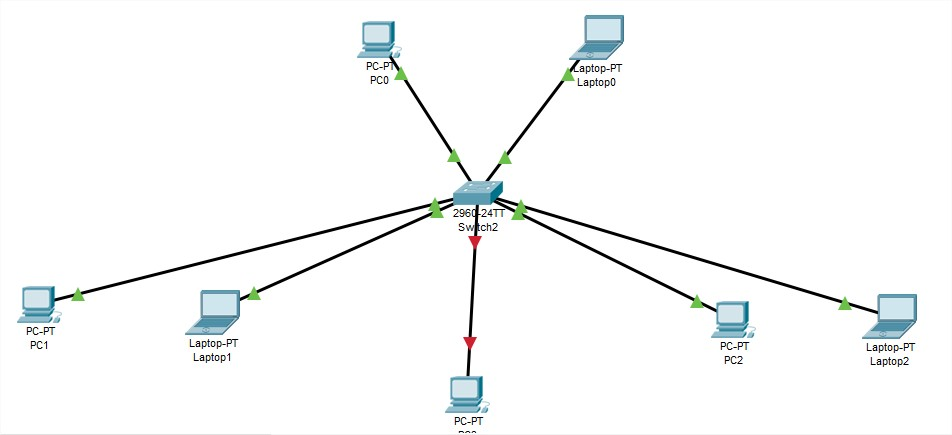
\includegraphics[scale=0.27]{red_prueba.jpg}
	\caption{Red de Prueba para VLANs en Packet Tracer}
\end{figure}

\section{\textbf{Manejo de Switches en eNSP}}
En ensp existen 2 tipos de vistas.
\begin{enumerate}
	\item Vista de usuario( <  > ).
	\item Vista de sistema( [ ] ): es el modo de configuración global.\\
	En cualquiera de las vistas para saber que comandos se pueden utilizar ingresamos el comando "?".
	Para ver las configuraciones actuales del switch ingresar el comando 
	\begin{lstlisting}[frame=single]
display current-configuration
	\end{lstlisting}
	
	Para entrar a la vista de sistema ingresamos:
	\begin{lstlisting}[frame=single]
system-view
	\end{lstlisting}
\end{enumerate}
\begin{enumerate}
	\item Asignar un nombre al switch.
	\begin{lstlisting}[frame=single]
sysname "nombre"
	\end{lstlisting}
	
	\item Asignar una contraseña. 
	\begin{lstlisting}[frame=single]
Aaa
local-user "usuario" 
password cipher "contrasena"
	\end{lstlisting}
	
	\item Crear vlan.
	\begin{lstlisting}[frame=single]
Vlan batch 2 3 // vlan 2 
	\end{lstlisting}
	
	\item Luego de creadas las VLANs debemos asignar los puertos físicos que van a estar asociados a cada VLAN, debemos acceder al puerto o rango de puertos que vamos a configurar en la interfaz, para esto ingresamos el siguiente comando:
	\begin{lstlisting}[frame=single]
interface Ethernet 0/0/\# 
	\end{lstlisting}
	
	\#  \textbf{es el número del puerto, en los puertos gigaethernet es el mismo procedimiento}
	\item Habilitamos cada puerto en modo acceso
	\begin{lstlisting}[frame=single]
port link-type Access
	\end{lstlisting}
	
	\item Asignamos el puerto a la vlan que se requiera:
	\begin{lstlisting}[frame=single]
port defaul vlan \#
	\end{lstlisting}
	
	\# \textbf{el numero de la vlan a la que se quiere asignar el Puerto.}
	
	\item Especificamos que los puertos estén encendidos (normalmente están encendidos pero para asegurarnos )
	\begin{lstlisting}[frame=single]
undo shutdown
	\end{lstlisting}
	
	\item Finalmente salimos de la vista de sistema con el comando:
	\begin{lstlisting}[frame=single]
quit
	\end{lstlisting}
	
	\item Y estando en la vista de usuario guardamos la configuración.
	\begin{lstlisting}[frame=single]
save
	\end{lstlisting}
	
	\item Para verificar que la configuración quedo guardada volvemos a  la vista de sistema y digitamos el comando:
	\begin{lstlisting}[frame=single]
display current-configuration
	\end{lstlisting}
	
\end{enumerate}

\newpage

\subsection{\textbf{Confirmar Configuración}}
Luego de realizada una configuración básica debemos de revisar que la configuración está correcta, para esto agregamos dispositivos a la red y los conectamos a diferentes puertos asociados a diferentes VLANs y no debe haber comunicación entre dispositivos de diferentes VLANs. \\

En la imagen \ref{ensp} se propone una red de prueba con cuatro VLANs diferentes:

\begin{figure}[ht]
	\centering
	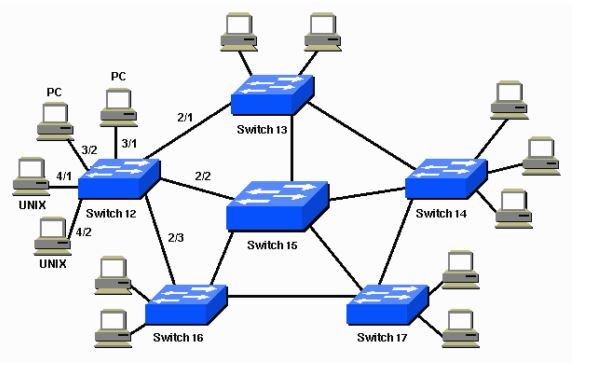
\includegraphics[scale=0.5]{2.jpg}
	\caption{Red de Prueba para VLANs en eNSP}
	\label{ensp}
\end{figure}

\section{Ejercicios}
\begin{itemize}
	\item Lectura previa de los protocolos SSH y STP
	\item Realizar una red WLAN con las mismas condiciones de la práctica anterior, solo en eNSP
\end{itemize}

Enviar la simulación a los correos \url{jujjaramillogr@unal.edu.co} y \url{klcerpac@unal.edu.co}, a ambos correos. Plazo hasta el sábado 16 de marzo de 2019.

\end{document}